\section{Schematy ideowe układu}
    \begin{figure}[!ht]
        \centering
        \scalebox{1}{\begin{subfigure}{\textwidth}
    \hspace{3cm}
    \begin{tikzpicture}
        \draw
            (0, 0) node[op amp, scale = 2](amp){} node[]{INA333}
            (amp) ++ (-1.66, -0.5) -- ++ (-1.22, 0) to[/tikz/circuitikz/bipoles/length=30pt, R, l=$R_G$, a=$10\ \Omega$] ++ (0, 1) -- ++ (1.22, 0)
            (amp.up) to[short, -o] ++ (0, 0.5) node[above]{$3.3\ V$}
            (amp.down) node[ground]{}
            (amp.+) -- ++ (-2.75, 0) to[R, l=$R_{meas}$, a=$100\ \Omega$] ++ (0, 1.96)
            (amp.-) -- ++ (-2.75, 0)
            (amp.+) ++ (-2.75, 0) to[short, *-o] ++ (0, -0.5) node[below]{$In_+$}
            (amp.-) ++ (-2.75, 0) to[short, *-o] ++ (0, 0.5) node[above]{$In_-$}

            (amp) ++ (1, -0.4) to[short, -o] ++ (0, -1) node[below]{$V_{REF}$}
            (amp.out) to[short, -o] ++ (1, 0) node[above]{$V_{out}$}

            (amp.+) ++ (-1, -2) node[below]{$V_{REF}$} to[R, o-*, l=$R_1$, a=$100\ k\Omega$] ++ (0, 2) 
        ;
    \end{tikzpicture}
\end{subfigure}
}
        \caption{Schemat ideowy wzmacniacza pomiarowego.}
        \label{sch:INA333}
    \end{figure}
    \begin{figure}[!ht]
        \centering
        \scalebox{1}{\begin{subfigure}{\textwidth}
    \hspace{0.5cm}
    \begin{tikzpicture}
        \draw
            (0, 0) node[op amp](amp){}
            (amp.up) to[short, -o] ++ (0, 0.5) node[above]{$3.3\ V$}
            (amp.down) node[ground]{}
            (amp.-) -| ++ (-0.5, 1.5) -| ++ (2.98, -2)
            (amp.out) -- ++ (0.1, 0) to[short, *-o] ++ (1, 0) node[above]{$V_{REF}$}
            (amp.out) ++ (0.1, -3) node[ground]{} to[C, l=$C_1$, a=$100\ nF$] ++ (0, 2) -- ++ (0, 1)
            (amp.+) -- ++ (-9, 0) ++ (0, -2) node[ground]{} to[C, l=$C_2$, a=$100\ nF$] ++ (0, 2)
            (amp.+) ++ (-6, -2) node[ground]{} to[C, -*, l=$C_3$, a=$1\ \mu F$] ++ (0, 2)
            (amp.+) ++ (-3, -2) node[ground]{} to[R, -*, l=$R_2$, a=$10\ k\Omega$] ++ (0, 2)
            to[R, -o, l=$R_1$, a=$10\ k\Omega$] ++ (0, 2) node[above]{$3.3\ V$}
        ;
    \end{tikzpicture}
\end{subfigure}}
        \caption{Schemat ideowy źródła napięcia referencyjnego.}
        \label{sch:Vref_gen}
    \end{figure}
    \begin{figure}[!ht]
        \centering
        \scalebox{1}{\begin{subfigure}{\textwidth}
    \hspace{3.5cm}
    \begin{tikzpicture}
        \draw
            (0, 0) node[ground]{} to[zDo, -*, l=$LM336$] ++ (0, 2) coordinate(out)
            to[R, -o, l=$R_1$, a=$820$] ++ (0, 2) node[above]{$3.3\ V$}
            (out) to[C, -o, l=$C_1$, a=$100\ nF$] ++ (3, 0) node[above]{$V_{out}$}
            (out) ++ (3.3, 0) node[circ, scale = 0.6]{}
            (out) ++ (3.5, 0) node[circ, scale = 0.6]{}
            (out) ++ (3.7, 0) node[circ, scale = 0.6]{}
            (out) ++ (5, 0) node[plain mono amp]{$?$}
        ;
    \end{tikzpicture}
\end{subfigure}}
        \caption{Schemat układu generacji szumu białego.}
        \label{sch:Noise_gen}
    \end{figure}
    \begin{figure}[!ht]
        \centering
        \scalebox{1}{    \begin{figure}[H]
        \centering
        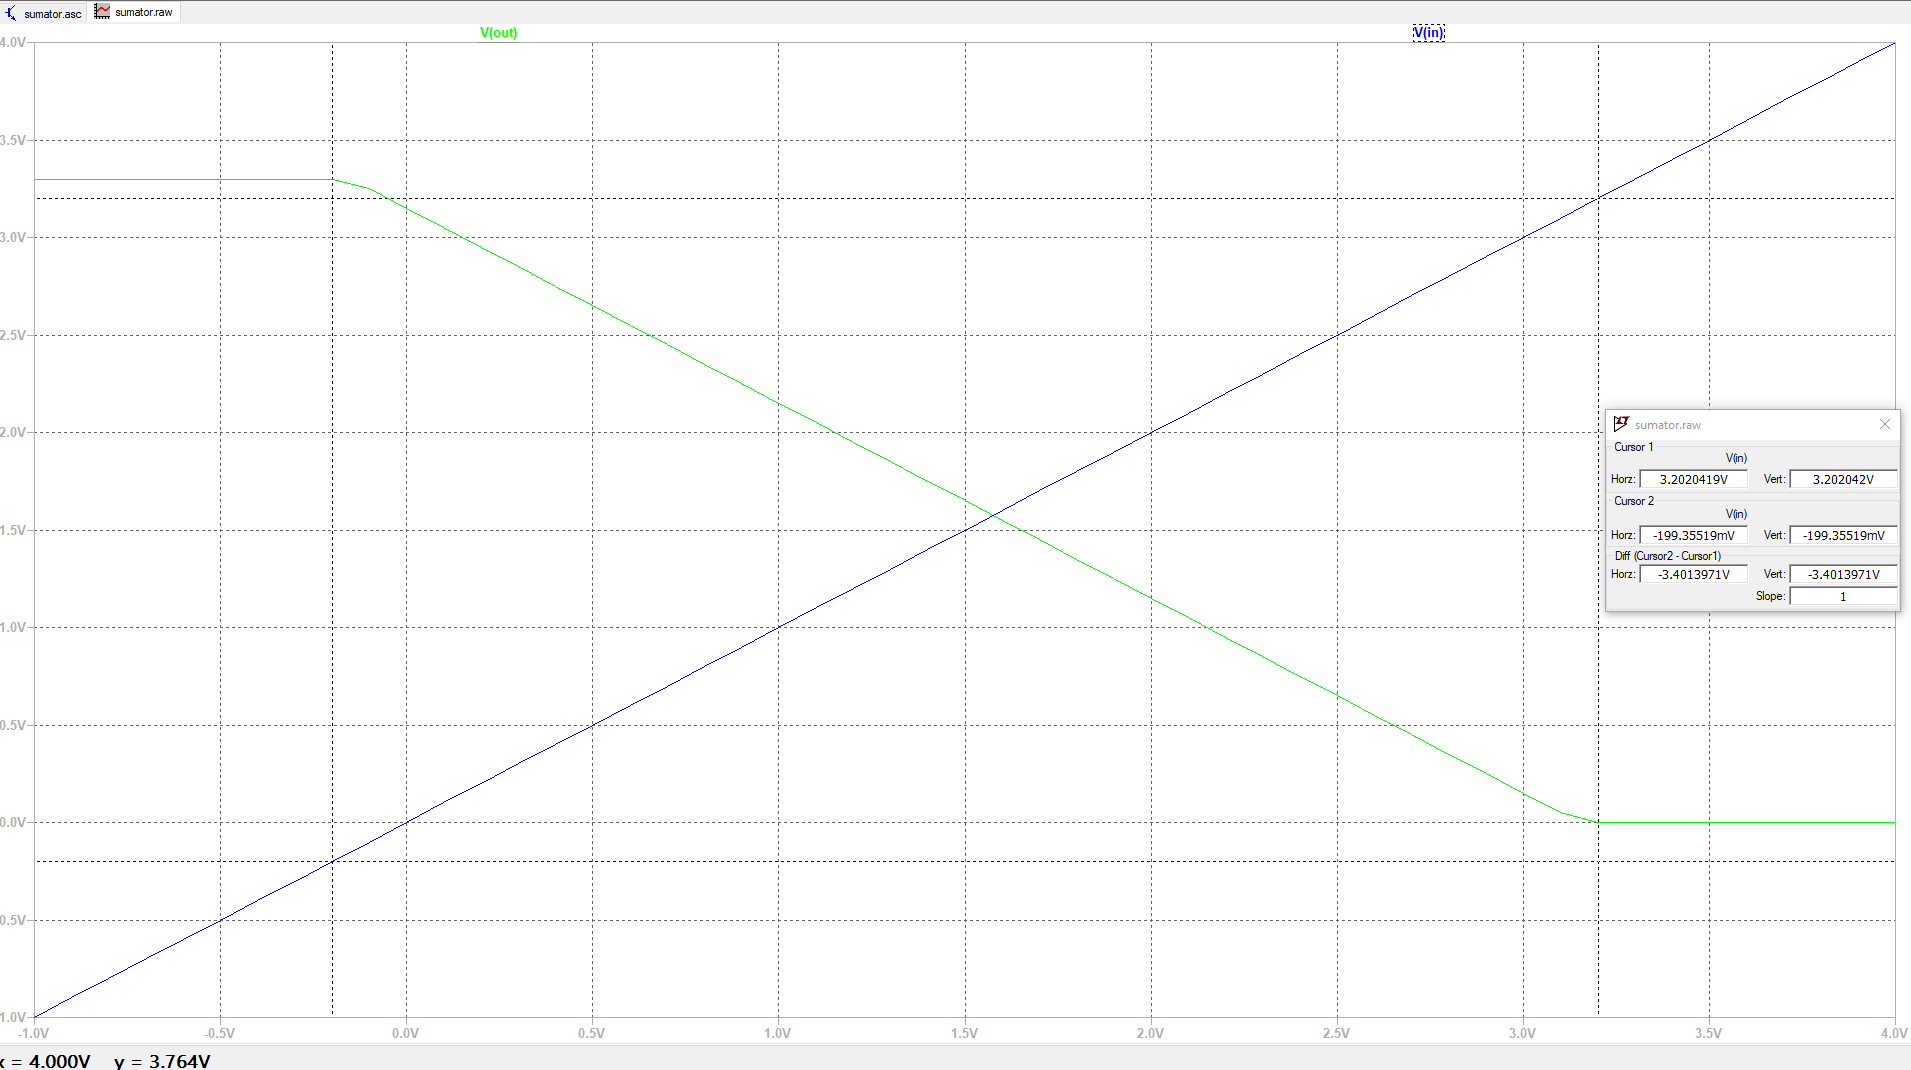
\includegraphics[width=1\linewidth]{images/sumator_dc.png}
        \caption{Symulacja dc układu sumującego, napięcia wyjściowego(Vout) od napięcia wejściowego (Vin)}
    \end{figure}}
        \caption{Układ sumacyjny dla dodania sygnału pomiarowego i szumu.}
        \label{sch:sumator}
    \end{figure}
    \begin{figure}[!ht]
        \centering
        \scalebox{1}{\begin{subfigure}{\textwidth}
    \hspace{4cm}
    \begin{tikzpicture}
    \draw
        (0, 0) node[draw, rectangle, minimum width = 3cm, minimum height = 3cm, label = {above:LT1117-3.3}](U1){}
        (U1.west) node[right=1mm] {IN}
        (U1.east) node[left=1mm] {OUT}
        (U1.south) node[above=1mm] {GND}
        (U1.south) node[ground]{}

        (U1.west) -- ++(-2,0) coordinate(IN)
        to[C, l=$C_{1}$, a=$10\ \mu$F] (IN |- U1.south) node[ground] {}
        (IN) to[short, -o] ++ (-1, 0) node[above]{$5V$}

        (U1.east) -- ++(2,0) coordinate(OUT)
        to[C, l=$C_{2}$, a=$100\ \mu$F] (OUT |- U1.south) node[ground] {}
        (OUT) to[short, -o] ++ (1, 0) node[above]{$3.3V$}

        ;
    \end{tikzpicture}
\end{subfigure}}
        \caption{Układ stabilizacji napięcia na 3.3V. }
        \label{sch:psu}
    \end{figure}